% split code (latex) parts into different files

% enhance listings

% "Deep Learning for Time Series Forecasting" by Jason Brownlee

% RNNs (Recurrent Neural Networks) (можно чуть чуть написать и сказать, что затронем 
% подробнее в следующей главе)

% LSTM (Long Short-Term Memory) (может пока не трогать, тк это модификация RNN)

% GRU (может пока не трогать, тк это модификация RNN)

% -------------

% topological intuition behind NN
% talk about backpropagation 
% universal approximation theorem (from Goodfellow)
% Manifold learning
% intuition behind thinking in n dimensions
% sigmoid/relu/softmax e.t.c. discussion for which is better
% parallel to neurobilogy
% architecture definition, main terms
% feed forward/not feed forward
% talk about gradient descent (stohastic, adam?)
% bayessian statistics? how is it different from classic 
% the idea of deriving cost functions from maximum likelihood
% maximum likelihood
% no free lunch theorem
% Regularization
% SVM and kernel trick
% cross entropy and Kullback–Leibler divergence

% --------------

% https://chatgpt.com/c/6817eeff-5420-8010-b35d-3c35fed4bdcf
% https://aistudio.google.com/prompts/1akCvM2Z46N9sApnbcqEbhtnS8eMy7HLz

% Part 1: Setting the Stage - What are we trying to do?
%     Introduction to Machine Learning & Supervised Learning

%     Intuition behind Thinking in n Dimensions

%     maybe drop:
%     (SVM & the kernel trick (how it bends space (later will be compared to nonlinearity in activation functions)))

%     What Is a Neural Network?
%     - Parallel to neurobiology
%     - Architecture definitions & main terms
%     - Feed‑forward vs. recurrent    

% Part 2: How Neural Networks "Compute"
%     How NNs “Fire”
%     - Activation functions(Sigmoid/ReLU/Softmax etc.):
%     (show how each nonlinearity “folds” space)
        
%     Geometric & Topological Intuition
%     - Manifold learning (quick review, mainly for intuition)
%     - topological intuition behind NN

% Part 3: How Neural Networks Learn
%     Cost functions (MSE, cross-entropy)

%     Probabilistic loss
%     - maximum likelihood 
%     - Deriving Cost Functions from Maximum Likelihood
%     (Cross‑entropy & Kullback–Leibler divergence (note: cross‑entropy ↔ KL divergence & MLE in one bullet))

%     Gradient descent mechanism (closed optimization, convex, e.t.c.)
%     Backpropagation
%     Optimization landscapes: local minima vs. saddle points (intuition).
%     Gradient Descent Variants (Stochastic, Mini-batch, Adam)

% Part 4: Theoretical & Practical Considerations
%     Universal Approximation Theorem
%     Overfitting and Underfitting
%     Regularization
%     Training, Validation, and Test Sets (hyperparameter tuning)
%     No Free Lunch Theorem

% Part 5: Bridging to RNNs
%     Limitations of Feed-Forward Networks for Sequences

% --------------

% Dimensionality reduction and visualisation of high dimensional data (https://colah.github.io/posts/2014-10-Visualizing-MNIST/)
% t-SNE

% \section{Рекуррентные нейронные сети}
\section{Глубокие сети}

\subsection{Что такое нейронная сеть? {\color{red} todo}}

В данной главе кратко вводятся основные понятия глубокого обучения. 
Сначала мы сформулируем методы мышления в многомерных измерениях. 
Затем рассмотрим модель перцептрона и закончим данную главу ознакомлением с 
архитектурой многослойного перцептрона (MLP), 
определив все, сопутствующие ему, основные термины.

Предполагается, что читатель уже знаком с основами классического машинного обучения, 
поэтому мы не будем подробно останавливаться на соответствующих понятиях.

\subsubsection{Интуиция мышления в n измерениях}

В процессе эволюции люди научились рассуждать в двух и трех измерениях. 
Приложив достаточно усилий, мы можем мыслить и в четырех измерениях. 
Машинное обучение часто требует от нас работы с тысячами измерений - 
или десятками тысяч, или миллионами. Даже очень простые вещи становится 
трудно понять, когда вы делаете их в очень большом количестве измерений.

Поэтому важно иметь в запасе методы для работы с такими данными. 
Люди, которые научились хорошо мыслить в высоких измерениях часто 
распологают, своего рода, ментальной библиотекой, содержащей множество 
различных техник. Возможно, эти техники не выделяются простотой, 
к которой мы привыкли при визуализации трех измерений, но, 
собрав библиотеку таких техник, вы сможете довольно хорошо научиться 
мыслить в высоких измерениях.

Рассмотрим несколько таких техник \cite{ndim_thinking}:

\begin{quoting}
    \itshape
    “Можно рассматривать высокоразмерное векторное пространство как 
    пространство состояний для системы со многими степенями свободы. 
    Например, мегапиксельное изображение - это точка в миллионном 
    векторном пространстве; изменяя изображение, можно исследовать 
    это пространство, и различные подмножества этого пространства 
    соответствуют различным классам изображений.

    Аналогичным образом можно интерпретировать звуковые волны, 
    коробку с газами, экосистему, совокупность избирателей, поток 
    цифровых данных, испытания случайных величин, результаты 
    статистического исследования, вероятностную стратегию в игре 
    двух игроков и многие другие конкретные объекты как состояния 
    в высокоразмерном векторном пространстве, а различные базовые 
    понятия, такие как выпуклость, расстояние, линейность, смена 
    переменных, ортогональность или внутреннее произведение, могут 
    иметь вполне естественные значения в некоторых из этих моделей 
    (хотя и не во всех).“
\end{quoting}

\begin{quoting}
    \itshape
    “Если вы пытаетесь представить себе некое 4D явление $P$, 
    сначала подумайте о соответствующем 3D явлении $P'$, 
    а затем представьте себя в роли 2D существа, которое 
    пытается представить себе $P'$. Преимущество в том, что, в отличие 
    от случая 4D vs. 3D, вы сами можете легко переключаться между 3D 
    и 2D перспективами и, следовательно, можете получить представление 
    о том, какая именно информация теряется, когда вы опускаете измерение. 
    (Можно назвать это «трюком Флатландии» ("Flatland trick"), в честь самого 
    известного литературного произведения, опирающегося на данную идею).“
\end{quoting}

\subsubsection{Нейронная сеть}

\paragraph{Перцептрон}

Нейронная сеть (neural network) строится из простейших элементов - искусственных 
нейронов. Одной из первых моделей такого нейрона был перцептрон, 
предложенный Фрэнком Розенблаттом в 1958 году \cite{Rosenblatt_perceptron}. Несмотря на то, что в 
современных архитектурах чаще используют сигмоидальные и ReLU-нейроны, 
понимание перцептрона важно для осознания эволюции подходов к обучению 
и архитектуре сетей.

% Как можно догадаться из названия, идея нейронных сетей была заимствована из нейробиологии 
% и вдохновлена работой мозга. Можно даже заметить сходство между структурой нейрона в мозге 
% и структурой перцептрона (см. рис. \ref{fig:neuron}).

% \begin{figure}[h!]
%     \centering
%     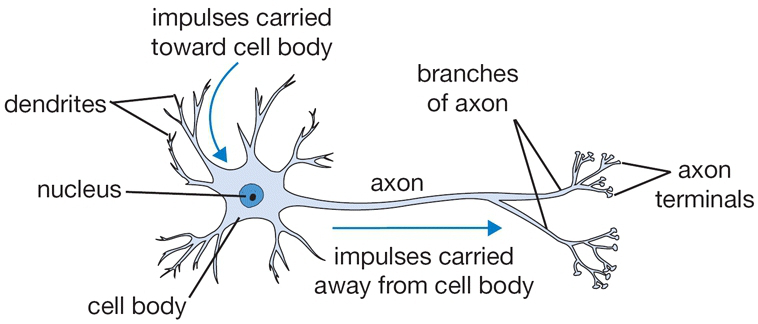
\includegraphics[width=0.49\textwidth, keepaspectratio]{neuron}
%     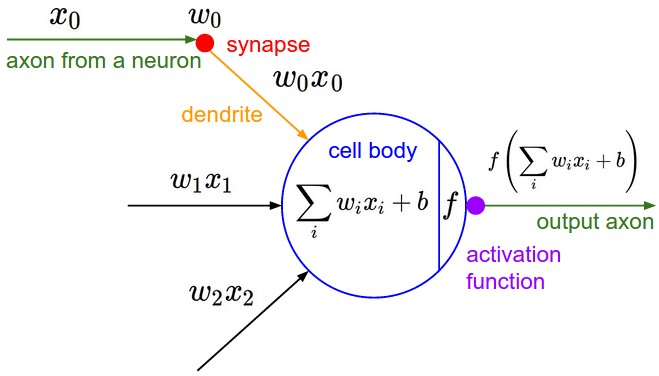
\includegraphics[width=0.49\textwidth, keepaspectratio]{neuron_model}
%     \caption{Рисунок биологического нейрона (слева) и его математической модели (справа)}
%     \label{fig:neuron}
% \end{figure}

Так как работает модель перцептрона? Перцептрон принимает на вход несколько бинарных значений: 
$x_1, x_2, ..., x_n $ и возвращает единственное бинарное значение:

\begin{figure}[h!]
    \centering
    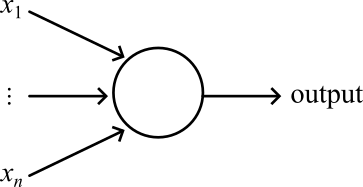
\includegraphics[width=0.4\textwidth, keepaspectratio]{perceptron}
    \caption{Модель перцептрона.}
    \label{fig:perceptron}
\end{figure}

Розенблатт предложил простую идею для расчета выходного значения. Он ввел понятие 
весов $w_1, w_2, ..., w_n$, действительных значений, отражающих важность каждого из, 
соответствующих входов. Выходное значение нейрона определяется из правила, превышает 
ли взвешенная сумма входов некоторое наперед заданное значение, называемое порогом 
(threshold):

\begin{equation*}
    \text{output} = \begin{cases}
        0 \quad \text{if} \quad \sum_j w_j x_j \leq \text{threshold} \\
        1 \quad \text{if} \quad \sum_j w_j x_j > \text{threshold} 
    \end{cases}
\end{equation*}

Однако, в машинном обучении чаще используют упрощенную версию данной записи. 
Перепишем $\sum_j w_j x_j$ в виде скалярного произведения, \hspace{20pt}
$\bm{w} \cdot \bm{x} \equiv \sum_j w_j x_j$, 
а порог заменим смещением (bias), $b \equiv -\text{threshold}$. Тогда наша запись примет вид:

\begin{equation*}
    \text{output} = \begin{cases}
        0 \quad \text{if} \quad \bm{w} \cdot \bm{x} + b \leq 0 \\
        1 \quad \text{if} \quad \bm{w} \cdot \bm{x} + b > 0 
    \end{cases}
\end{equation*}

Одним из примеров применения перцептрона может послужить вычисление логических функций.
Так, например, рассмотрим перцептрон, у которого всего два входа, $x_1, x_2 \in \left\{ 0, 1 \right\}$. 
И вручную примем $w_1 = w_2 = -2, \quad b = 3$. Тогда наш перцептрон примет вид:

\begin{figure}[h!]
    \centering
    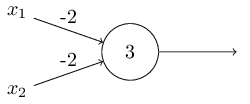
\includegraphics[width=0.4\textwidth, keepaspectratio]{perceptron2}
    \caption{Пример перцептрона с весами $\bm{w} = \left[ -2 \hspace{3pt} -2 \right]^T$ и 
    смещением $b = 3$.}
    \label{fig:perceptron2}
\end{figure}

При $\bm{x} = \left[ 0 \hspace{3pt} 0 \right]^T$, получим $1$, т.к. 
$\bm{w} \cdot \bm{x} + b = (-2) \cdot 0 + (-2) \cdot 0 + 3 = 3 > 0$.
Построим таблицу всех значений:

\begin{minipage}{0.4\textwidth}
    \centering
    \renewcommand{\arraystretch}{1.5}
    \begin{tabular}{ccc}
        $x_1$ & $x_2$ & $f$ \\
        \midrule
        0 & 0 & 1 \\
        0 & 1 & 1 \\
        1 & 0 & 1 \\
        1 & 1 & 0 \\
    \end{tabular}
    \captionof{table}{Значения, которые принимает перцептрон (\ref{fig:perceptron2}) 
    при различных значениях $x_1, x_2 \in \left\{ 0, 1 \right\}$.}
    \label{tab:perceptron-values}
\end{minipage}
\hspace{30pt}
\begin{minipage}{0.4\textwidth}
    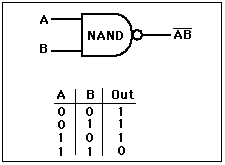
\includegraphics[width=\linewidth]{NAND}
    \captionof{figure}{Штрих Шеффера (NAND gate).}
    \label{fig:NAND}
\end{minipage}\\

Таким образом, наш перцептрон реализует Штрих Шеффера (NAND gate). 
Исходя из этого примера видно, что мы можем использовать перцептроны для 
расчета простых логических функций. Вообще говоря, мы можем рассчитать любую логическую 
(и не только, см. {\color{red} главу...}) функцию, 
используя сеть из перцептронов, называемаю нейронной сетью.

\paragraph{Архитектура нейронной сети}

Нейронная сеть состоит из композиции нейронов (т.е. когда в качестве входов для 
нейронов используются выходы других нейронов), например:

\begin{figure}[h!]
    \centering
    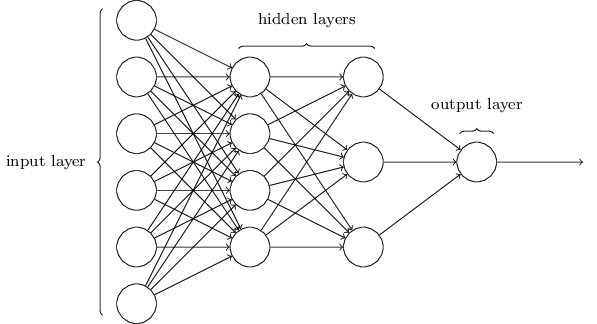
\includegraphics[width=0.8\textwidth, keepaspectratio]{NN_example1}
    \caption{Архитектура простой нейронной сети.}
    \label{fig:NN1}
\end{figure}

Самый левый слой называется \textit{входным слоем (input layer)}, а нейроны в нем 
называются \textit{входными нейронами (input neurons)}. Самый правый, или же 
\textit{выходной слой (output layer)} содержит в себе 
\textit{выходные нейроны (output neurons)}. Слои между ними называются 
\textit{скрытыми (hidden layers)}. Количество скрытых слоев определяет 
\textit{глубину (depth)} нейронной сети, а размерность скрытых слоев 
определяет \textit{ширину (width)} модели.

Подобные сети называют \textit{многослойными перцептронами (MLPs)}. (Исторически пошло, 
что иногда их так называют даже когда они состоят не из перцептронов). 

\paragraph{feedforward vs recurrent}

До сих пор мы обсуждали нейронные сети, в которых выход из одного слоя используется как 
вход для следующего. Подобные сети называются \textit{нейронными сетями прямого распространения 
(feedforward neural networks)}. Это значит, что у нас нет циклов в сети - информация всегда 
поступает вперед и никогда не возвращается назад.

Однако существуют и другие модели искусственных нейронных сетей, 
в которых возможны циклы обратной связи. Подобные модели называются 
\textit{рекуррентными нейронными сетями (recurrent neural networks)} 
(см. {\color{red} главу...}). 
Идея этих моделей заключается в 
том, что нейроны работают в течение некоторого ограниченного периода 
времени, а затем затихают. Это возбуждение может стимулировать другие 
нейроны, которые через некоторое время также возбуждаются на ограниченное 
время. Это заставляет еще большее количество нейронов срабатывать, и 
так со временем мы получаем каскад нейронов, которые срабатывают. Циклы 
в такой модели не вызывают проблем, так как выход нейрона влияет на его 
вход только через некоторое время, а не мгновенно \cite{NN_Nielsen}.

\subsection{Как нейронные сети «вычисляют»?}

\subsubsection{Функции активации}

До сих пор, мы подбирали параметры вручную. Однако, у нас возникли бы серьезные 
проблемы, если бы мы захотели подобрать параметры к, например, следующей нейронной сети:
\newpage

\begin{figure}[h!]
    \centering
    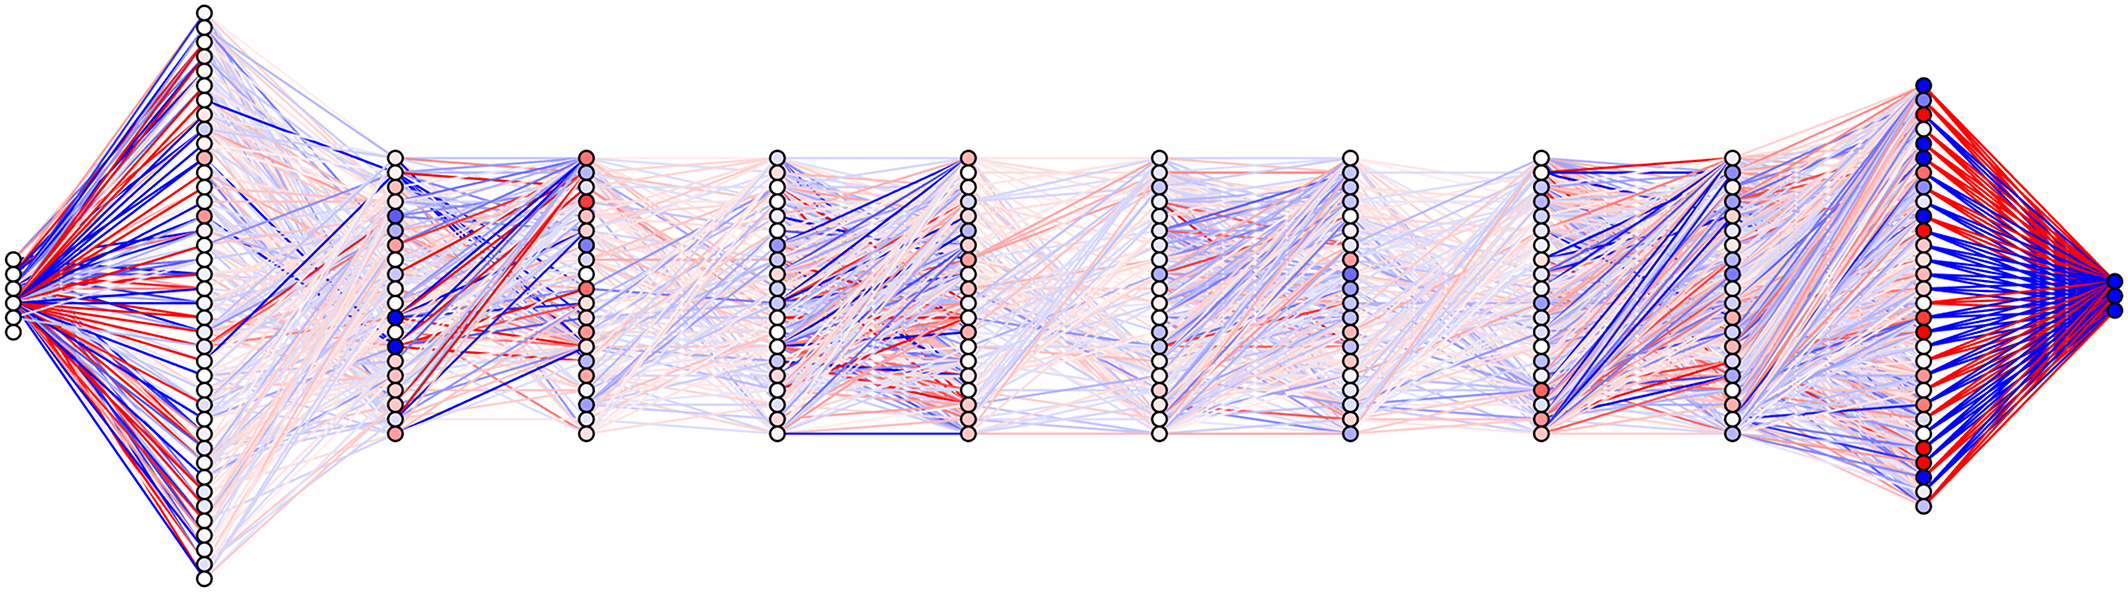
\includegraphics[width=1\textwidth, keepaspectratio]{NN_example3}
    \caption{Архитектура нейронной сети.}
    \label{fig:NN3}
\end{figure}

Которая, вообще говоря, считается относительно небольшой по современным меркам 
(ходят слухи, что модель GPT-4 насчитывает $\sim 1.8$ триллионов параметров в 
120 слоях \cite{gpt4_architecture}).

Однако ситуация лучше, чем кажется на первый взгляд. 
Проектирование и обучение нейронной сети не сильно отличается от обучения 
любой другой модели машинного обучения с помощью градиентного спуска. 

Таким образом, мы возвращаеся к проблеме перцептронов с жёсткой (ступенчатой) 
функцией активации:
\begin{equation*}
    \text{output} = \begin{cases}
        0 \quad \text{if} \quad \bm{w} \cdot \bm{x} + b \leq 0 \\
        1 \quad \text{if} \quad \bm{w} \cdot \bm{x} + b > 0 
    \end{cases}
\end{equation*}

Хотя такая модель достаточно проста, её основное ограничение в том, 
что функция активации не является дифференцируемой в точке разрыва, 
а её производная равна нулю везде, где она определена. 
Из-за этого градиентный спуск применять невозможно: градиент отсутствует или 
обращается в ноль, и веса не обновляются.

\paragraph{Сигмоидальные блоки}

На помощь приходит новый вид искусственных нейронов, называемый 
\textit{сигмоидальным (sigmoid neuron)} (далее будем называть просто сигмоидом). 
Основное отличие от перцептрона заключается в том, что
сигмоид может вернуть любое значение из интервала от 0 до 1, 
задаваемое гладкой, непрерывно дифференцируемой функцией $\sigma$, 
называемой сигмоидальной функцией:
\begin{equation*}
    \sigma(z) \defeq \cfrac{1}{1 + e^{-z}}
\end{equation*}

Таким образом функция активации принимает вид:
\begin{equation*}
    \text{output} = \sigma(\bm{wx} + b) = \cfrac{1}{1 + e^{-\bm{wx} - b}}
\end{equation*}

Если мы посмотрим на графики функций активации перцептрона и сигмоида, то 
заметим, что сигмоидальная функция это просто сглаженная версия ступенчатой 
(Вообще говоря, при $\bm{wx + b = 0}$ перцептрон возвращает 0, а ступенчатая 
функция 1. Так что строго говоря ступенчатую функцию следовало бы изменить в 
этой одной точке, чтобы ее можно было называть функцией активации перцептрона, но 
суть понятна).

\begin{minipage}{0.4\textwidth}
    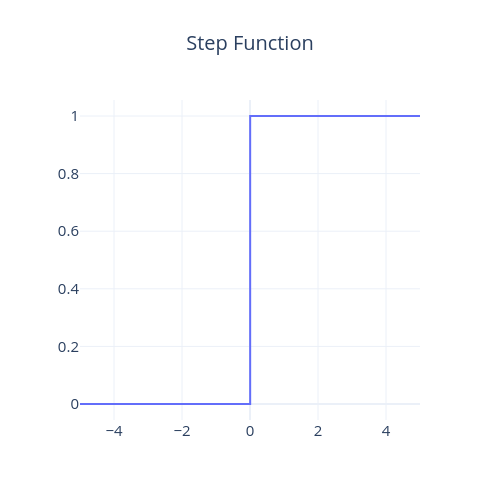
\includegraphics[width=\linewidth]{step}
    \captionof{figure}{График ступенчатой функции.}
    \label{fig:step}
\end{minipage}
\hspace{30pt}
\begin{minipage}{0.4\textwidth}
    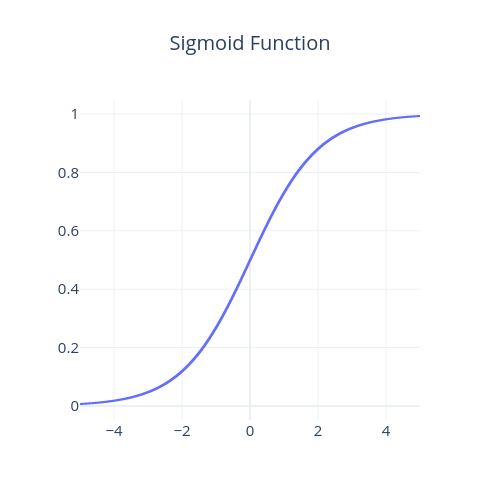
\includegraphics[width=\linewidth]{sigma}
    \captionof{figure}{График сигмоидальной функции.}
    \label{fig:sigma}
\end{minipage}\\

Иногда вместо сигмоидальной функции используют гиперболический тангенс\\ 

\begin{minipage}{0.4\textwidth}
    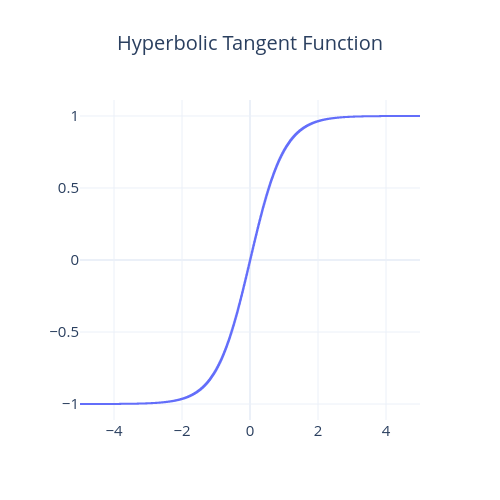
\includegraphics[width=\linewidth]{tanh}
    \captionof{figure}{График гиперболического тангенса.}
    \label{fig:tanh}
\end{minipage}
\hspace{30pt}
\begin{minipage}{0.3\textwidth}
    \begin{equation*}
        \text{tanh}(z) \defeq \cfrac{e^{2z} - 1}{e^{2z} + 1}
    \end{equation*}
\end{minipage}\\

Эти функции активации тесно связаны: $\text{tanh}(z) = 2 \sigma(2z) - 1$.

Однако, сигмоидальные блоки близки к асимптоте в большей части своей области определения -
приближаются к высокому значению, когда $z$ стремится к бесконечности, и к низкому,
когда $z$ стремится к минус бесконечности. Высокой чувствительностью они обладают 
только в окрестности нуля. Из-за насыщения сигмоидальных блоков градиентное
обучение сильно затруднено. Поэтому использование их в качестве скрытых блоков
в сетях прямого распространения ныне не рекомендуется. Применение же в качестве
выходных блоков совместимо с обучением градиентными методами, если функция
стоимости компенсируется насыщением сигмоиды в выходном слое.

Сигмоидальные функции активации все же применяются, но не в сетях прямого
распространения. К рекуррентным сетям, многим вероятностным моделям и некоторым 
автокодировщикам предъявляются дополнительные требования, исключающие
использование кусочно-линейных функций активации и делающие сигмоидальные
блоки более подходящими, несмотря на проблемы насыщения.

\paragraph{Блоки линейной ректификации}

В качестве функции активации по умолчанию для большинства нейронных сетей прямого 
распространения рекомендуется ректифицированная линейная функция активации (ReLU):

\begin{minipage}{0.45\textwidth}
    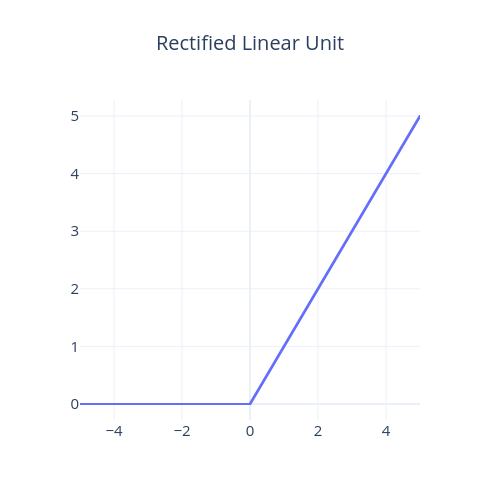
\includegraphics[width=\linewidth]{ReLU}
    \captionof{figure}{График ректифицированной линейной функции.}
    \label{fig:ReLU}
\end{minipage}
\hspace{30pt}
\begin{minipage}{0.2\textwidth}
    \begin{align*}
        \text{ReLU}(z) &= z^{+} \\
        &= \text{max}(0, z) \\
        &= \cfrac{z + |z|}{2} \\[0.5em]
        &= \begin{cases}
            z \quad \text{if} \quad z > 0, \\
            0 \quad \text{if} \quad z \leq 0
        \end{cases}
    \end{align*}
\end{minipage}\\

Применение ее к выходу линейного преобразования дает нелинейное преобразование. 
Функция, впрочем, очень близка
к линейной - она является кусочно-линейной с двумя линейными участками. 
Поскольку блоки линейной ректификации почти линейны, сохраняются
многие свойства, благодаря которым линейные модели легко поддаются
оптимизации градиентными методами. Сохраняются также свойства, обес­печивающие 
хорошую обобщаемость линейных моделей. Общий принцип
информатики - строить сложные системы из минимальных компонентов.
От памяти машины Тьюринга требуется только способность хранить нуль
и единицу, а универсальный аппроксиматор можно построить из ректифи-
цированных линейных функций \cite{Goodfellow-et-al-2016}.

\paragraph{Нелинейность}

После того как мы познакомились с различными функциями активации, 
возникает естественный вопрос: зачем нужны именно нелинейные активации? 
Ведь линейные функции легко оптимизировать методом градиентного спуска. 
Дело в том, что композиция любых линейных преобразований остаётся линейной 
функцией входа. 

Пусть у нас есть две кривые линии на плоскости и задача нейронной сети заключается в том, 
чтобы классифицировать к которой из двух кривых принадлежит та или иная точка. В случае 
линейной модели, мы бы не добились особого успеха, тк наши кривые линейно неразделимы:\\

\begin{minipage}{0.35\textwidth}
    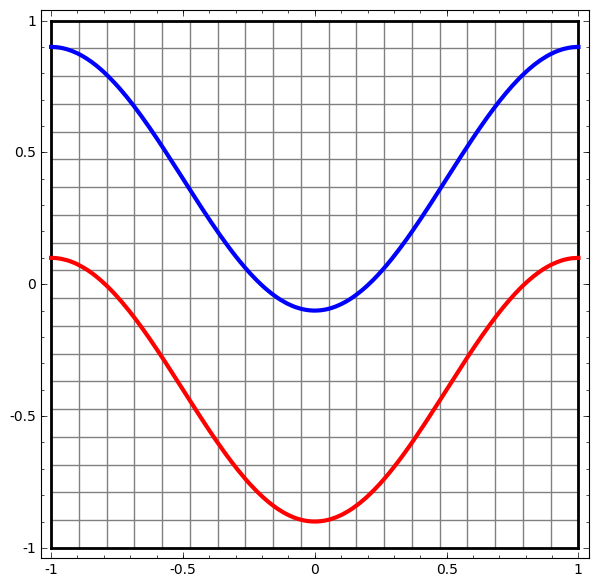
\includegraphics[width=\linewidth]{colah1}
    \label{fig:colah1}
\end{minipage}
\hspace{80pt}
\begin{minipage}{0.35\textwidth}
    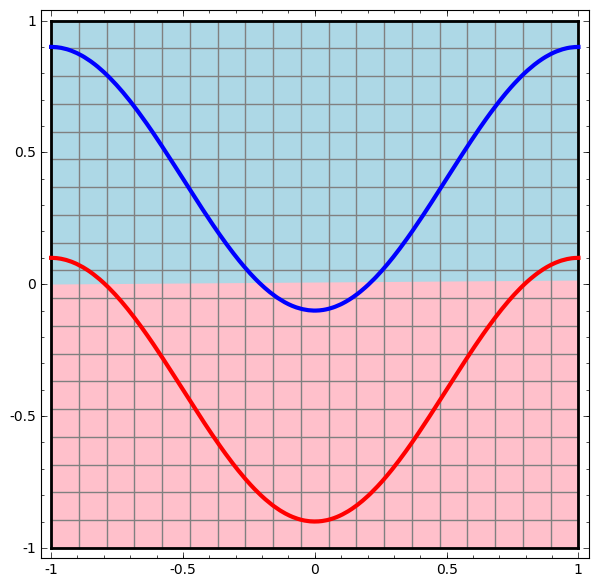
\includegraphics[width=\linewidth]{colah2}
    \label{fig:colah2}
\end{minipage}\\

Однако, если перед классификацией, мы преобразуем наши данные 
(в данном случае, с применением сигмоидальной функции), 
то получим их \textit{представление (representation)} в 
пространстве, в котором их уже легче классифицировать \cite{colah}:

\begin{figure}[h!]
    \centering
    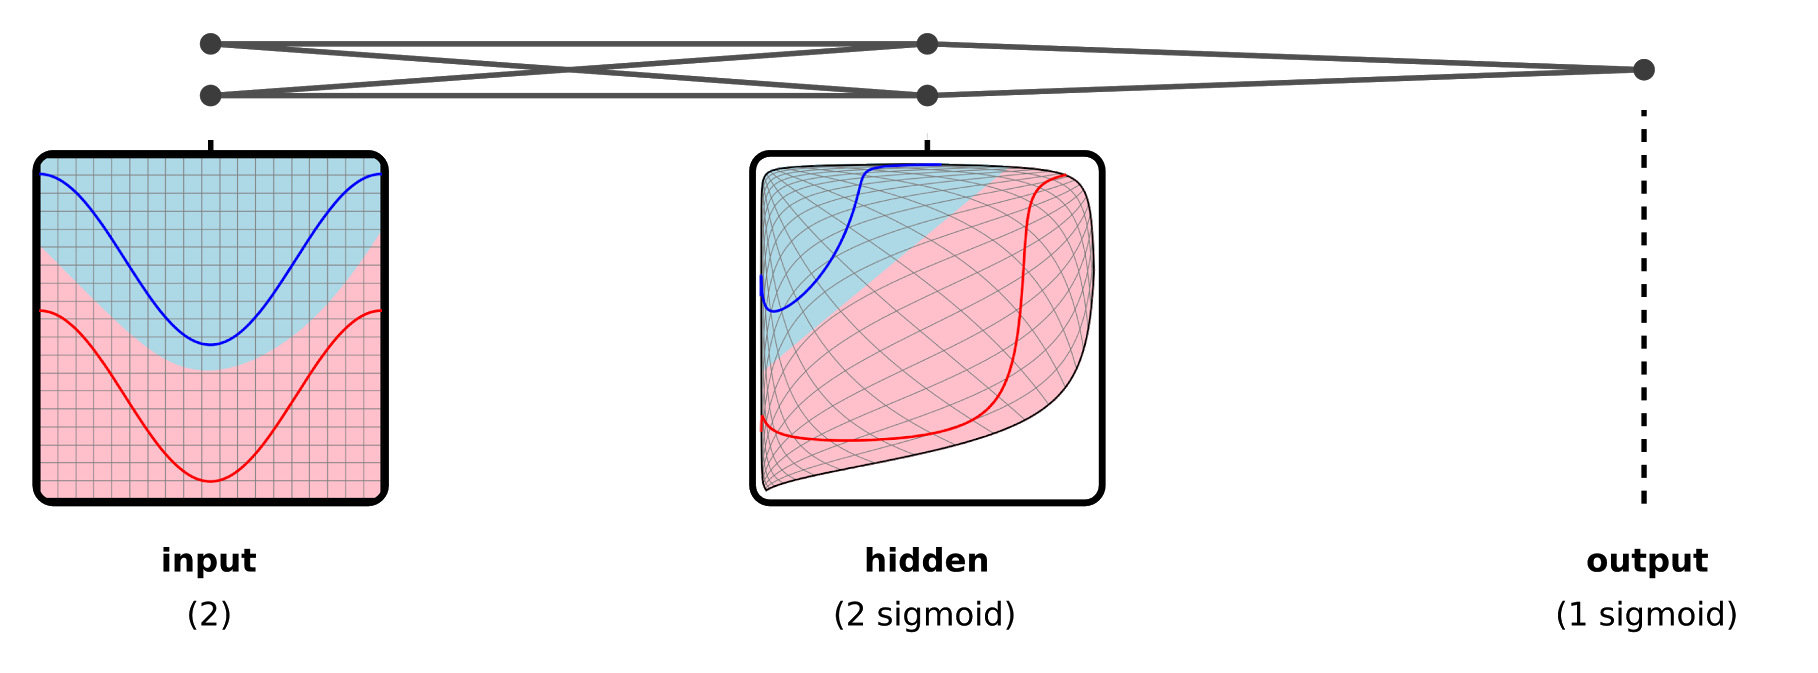
\includegraphics[width=1\textwidth, keepaspectratio]{colah3}
    \caption{Иллюстрация того, как нелинейный слой «разворачивает» 
    данные в новом пространстве признаков, делая их линейно разделимыми.}
    \label{fig:colah3}
\end{figure}

\subsubsection{Многообразия и топология {\color{red} todo}}

% leave for later

\subsection{Как нейронные сети обучаются?}

\subsubsection{Функции стоимости}

